\documentclass[aspectratio=169,10pt]{beamer}

\usepackage{ctex}
\usepackage{graphicx}
\usepackage{xcolor}
\usepackage{booktabs}
\usepackage{tabularx}

\usetheme{default}
\setbeamertemplate{navigation symbols}{}
\setbeamertemplate{footline}[frame number]
\setbeamersize{text margin left=8mm,text margin right=8mm}
\graphicspath{{docs/slides/screenshots/}{screenshots/}}

\definecolor{MTRBlue}{RGB}{31, 58, 89}
\definecolor{MTRRed}{RGB}{180, 32, 45}
\definecolor{MTRPurple}{RGB}{109, 40, 217}
\definecolor{SoftGray}{RGB}{245, 247, 250}
\definecolor{TextGray}{RGB}{45, 55, 72}

\setbeamercolor{title}{fg=MTRBlue}
\setbeamercolor{frametitle}{fg=MTRBlue}
\setbeamercolor{normal text}{fg=TextGray}
\setbeamercolor{block title}{fg=white,bg=MTRBlue}
\setbeamercolor{block body}{fg=TextGray,bg=SoftGray}
\setbeamercolor{alerted text}{fg=MTRRed}
\setbeamertemplate{itemize item}{\color{MTRRed}\small$\blacktriangleright$}
\setbeamertemplate{itemize subitem}{\color{MTRBlue}\scriptsize$\bullet$}
\renewcommand{\arraystretch}{1.18}

\newcommand{\hciprinciple}[1]{\vspace{0.25em}\textcolor{MTRPurple}{\small\textbf{对应 HCI 原则：}#1}}
\newcommand{\speakerline}[2]{\centering{\Huge\bfseries #1}\\[0.8em]{\Large 学号：#2}\\[1.2em]}

\title{港铁票价优化器与综合交通交互系统}
\subtitle{MTR Fare Optimizer \& Transit Interface}
\author{同济大学《人机交互导论》课程大作业}
\date{}

\begin{document}

\begin{frame}
  \titlepage
  \vspace{-1.2em}
  \begin{columns}[T,onlytextwidth]
    \begin{column}{0.48\textwidth}
      \small
      \begin{tabular}{ll}
        组长 & 李堂辉 2351078 \\
        组员 & 高胜寒 2351837 \\
        组员 & 郎若谷 2351871 \\
        组员 & 樊祺 2350262 \\
      \end{tabular}
    \end{column}
    \begin{column}{0.48\textwidth}
      \small
      GitHub 开源仓库：\href{https://github.com/Tanghui-Li/MTR-fare-optimizer/}{Tanghui-Li/MTR-fare-optimizer}\\
      在线部署：\href{https://mtr-optimizer.shgao.top}{mtr-optimizer.shgao.top}\\
      欢迎课后访问和试用。
    \end{column}
  \end{columns}
\end{frame}

\begin{frame}{汇报结构与任务主线}
  \begin{columns}[T,onlytextwidth]
    \begin{column}{0.50\textwidth}
      \begin{block}{从粉岭站问题开始}
        罗湖 $\to$ 屯门，成人八达通：常规 HK\$59.2；在东铁线粉岭站出闸再入闸后总价 HK\$51.5，节省 HK\$7.7。
      \end{block}
      \begin{itemize}
        \item 这个结果难以由一条固定规则推导，需要查询票价矩阵并枚举候选断点。
        \item 主流地图软件通常按时间、换乘和步行距离规划路线，本项目补齐按港铁票价优化的查询入口。
        \item 系统同时解释“怎么走”“多少钱”“为什么这样走”。
      \end{itemize}
    \end{column}
    \begin{column}{0.47\textwidth}
      \begin{block}{四个汇报部分}
        \begin{itemize}
          \item 李堂辉：项目背景与路由算法
          \item 高胜寒：界面设计、移动端适配、线路显示
          \item 郎若谷：站点周边景点与美食推荐
          \item 樊祺：无障碍设施信息与用户体验调研
        \end{itemize}
      \end{block}
      \hciprinciple{以用户为中心设计：从真实任务出发组织信息架构和交互流程。}
    \end{column}
  \end{columns}
\end{frame}

\begin{frame}{李堂辉：项目背景与设计目标}
  \begin{columns}[T,onlytextwidth]
    \begin{column}{0.56\textwidth}
      \begin{itemize}
        \item 香港交通网络复杂，直观路线的票价可能高于分段出入闸方案。
        \item 用户真正关心的是：花多少钱、怎么走、在哪里换乘、是否需要额外出入闸。
        \item 除地图上的线路走向几何校正外，站点、票价、设施和实时交通数据均基于香港政府开放资料 data.gov.hk。
        \item 项目已开源在 GitHub：\href{https://github.com/Tanghui-Li/MTR-fare-optimizer/}{Tanghui-Li/MTR-fare-optimizer}，并部署在 \href{https://mtr-optimizer.shgao.top}{mtr-optimizer.shgao.top}。
      \end{itemize}
      \hciprinciple{尼尔森启发式“系统与现实世界匹配”：用真实站点、线路、票价和设施降低理解成本。}
    \end{column}
    \begin{column}{0.40\textwidth}
      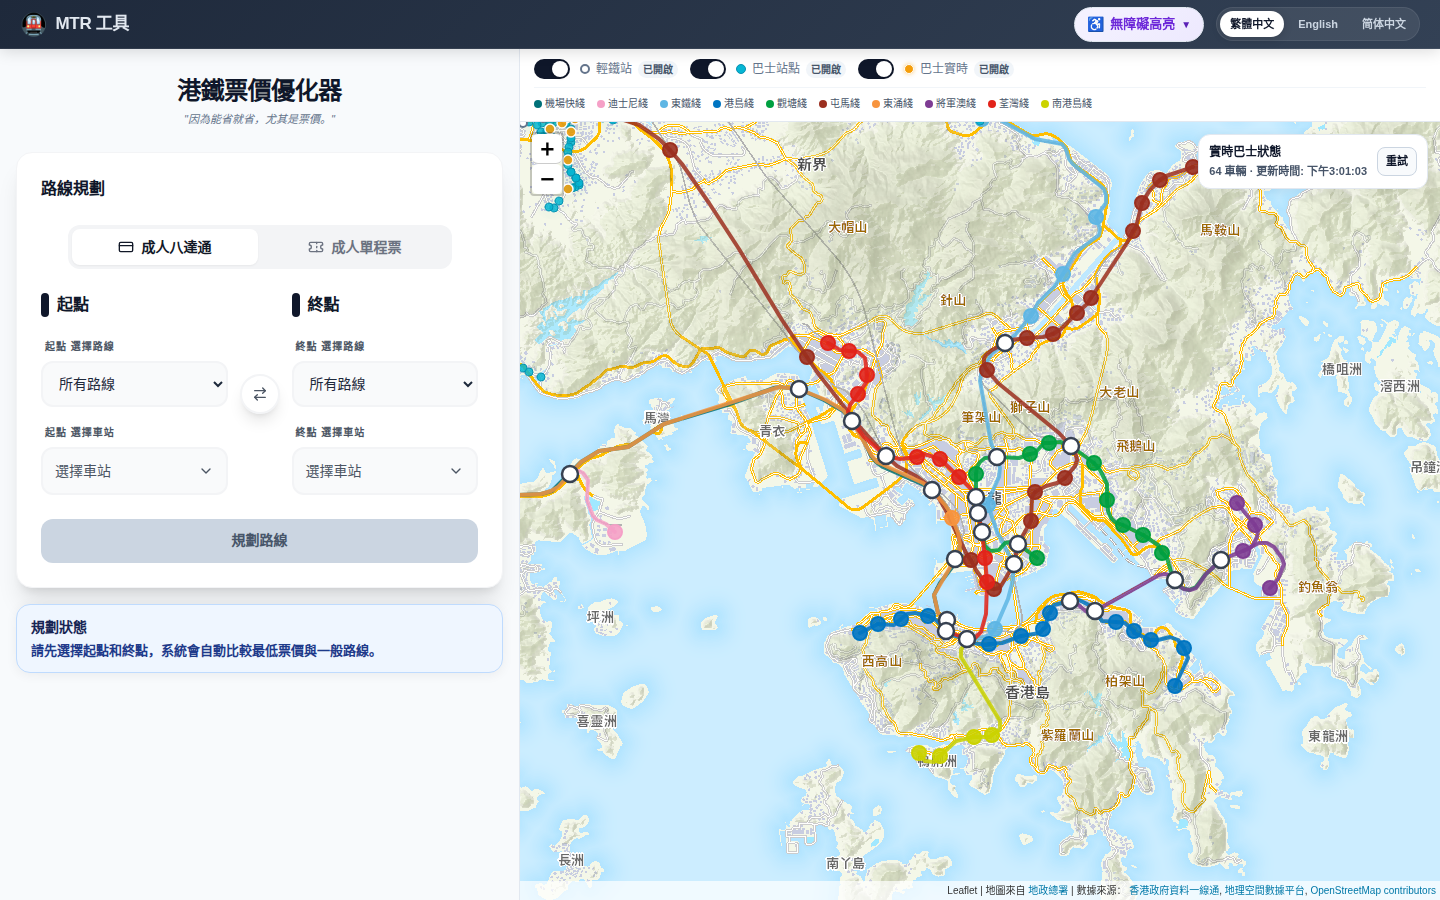
\includegraphics[width=\linewidth,height=0.68\textheight,keepaspectratio]{desktop-map-overview.png}
    \end{column}
  \end{columns}
\end{frame}

\begin{frame}{数据基础：从开放数据到统一交通图}
  \begin{columns}[T,onlytextwidth]
    \begin{column}{0.46\textwidth}
      \begin{block}{输入数据}
        \begin{itemize}
          \item 港铁线路与站点：data.gov.hk 原始 CSV
          \item 成人八达通 / 单程票票价矩阵
          \item 机场快线、轻铁、港铁巴士数据
          \item 车站无障碍设施与实时交通接口
        \end{itemize}
      \end{block}
    \end{column}
    \begin{column}{0.50\textwidth}
      \begin{block}{统一建模}
        \begin{itemize}
          \item 节点：车站、轻铁站、巴士站、换乘点
          \item 边：乘车、换乘、出闸再入闸、接驳关系
          \item 权重：票价、时间、换乘和操作复杂度
        \end{itemize}
      \end{block}
      \begin{center}
        \small
        开放数据 $\to$ 清洗归一 $\to$ 统一交通图 $\to$ 路径搜索 $\to$ 可解释界面
      \end{center}
    \end{column}
  \end{columns}
  \hciprinciple{尼尔森启发式“系统状态可见性”：数据来源、建模过程和输出规则需要让用户可感知。}
\end{frame}

\begin{frame}{路由算法：票价优化超过最短路}
  \begin{columns}[T,onlytextwidth]
    \begin{column}{0.48\textwidth}
      \begin{block}{计算流程}
        \begin{itemize}
          \item 输入：起点、终点、票种
          \item 构图：按票种选择对应票价矩阵
          \item 搜索：计算普通路线与分段票价优化路线
          \item 输出：总票价、分段路线、站点序列、线路标签、出入闸说明
        \end{itemize}
      \end{block}
    \end{column}
    \begin{column}{0.48\textwidth}
      \begin{block}{为什么要分段展示}
        \begin{itemize}
          \item 票价优化可能要求用户出闸再入闸
          \item 单一金额无法说明可执行步骤
          \item 分段卡片把“算法结果”转化为“用户能照做的步骤”
        \end{itemize}
      \end{block}
    \end{column}
  \end{columns}
  \hciprinciple{尼尔森启发式“识别优于回忆”：把站点序列和出入闸动作直接展示，避免用户记忆隐藏规则。}
\end{frame}

\begin{frame}{回到粉岭：算法正确性与可解释性}
  \begin{columns}[T,onlytextwidth]
    \begin{column}{0.52\textwidth}
      \begin{block}{查询：罗湖 $\to$ 屯门，成人八达通}
        \begin{tabularx}{\linewidth}{lXr}
          \toprule
          方案 & 乘车分段 & 票价 \\
          \midrule
          常规 & 罗湖 $\to$ 屯门 & HK\$59.2 \\
          分段 & 罗湖 $\to$ 粉岭 & HK\$26.5 \\
          分段 & 粉岭 $\to$ 屯门 & HK\$25.0 \\
          \midrule
          优化 & 粉岭出闸再入闸 & HK\$51.5 \\
          \bottomrule
        \end{tabularx}
      \end{block}
      \begin{block}{结果}
        节省 HK\$7.7；粉岭站位于东铁线，是本次票价断点。
      \end{block}
    \end{column}
    \begin{column}{0.44\textwidth}
      \begin{block}{为什么需要查询系统}
        \begin{itemize}
          \item 港铁票价矩阵存在区间、过境站和换乘组合影响。
          \item “在哪一站出闸再入闸更便宜”无法用一条简单规则概括。
          \item 需要枚举候选断点并比较总票价。
          \item 通用地图软件通常提供最快或少换乘路线，缺少按票价筛选。
        \end{itemize}
      \end{block}
    \end{column}
  \end{columns}
\end{frame}

\begin{frame}{第二部分：界面设计}
  \speakerline{高胜寒}{2351837}
  \begin{block}{负责内容}
    移动端适配、线路显示、路线结果表达、地图图层与整体界面可用性。
  \end{block}
  \hciprinciple{诺曼执行-评估循环：界面需要支持用户形成目标、执行操作、理解反馈。}
\end{frame}

\begin{frame}{桌面端信息架构：规划与地图并列}
  \begin{columns}[T,onlytextwidth]
    \begin{column}{0.60\textwidth}
      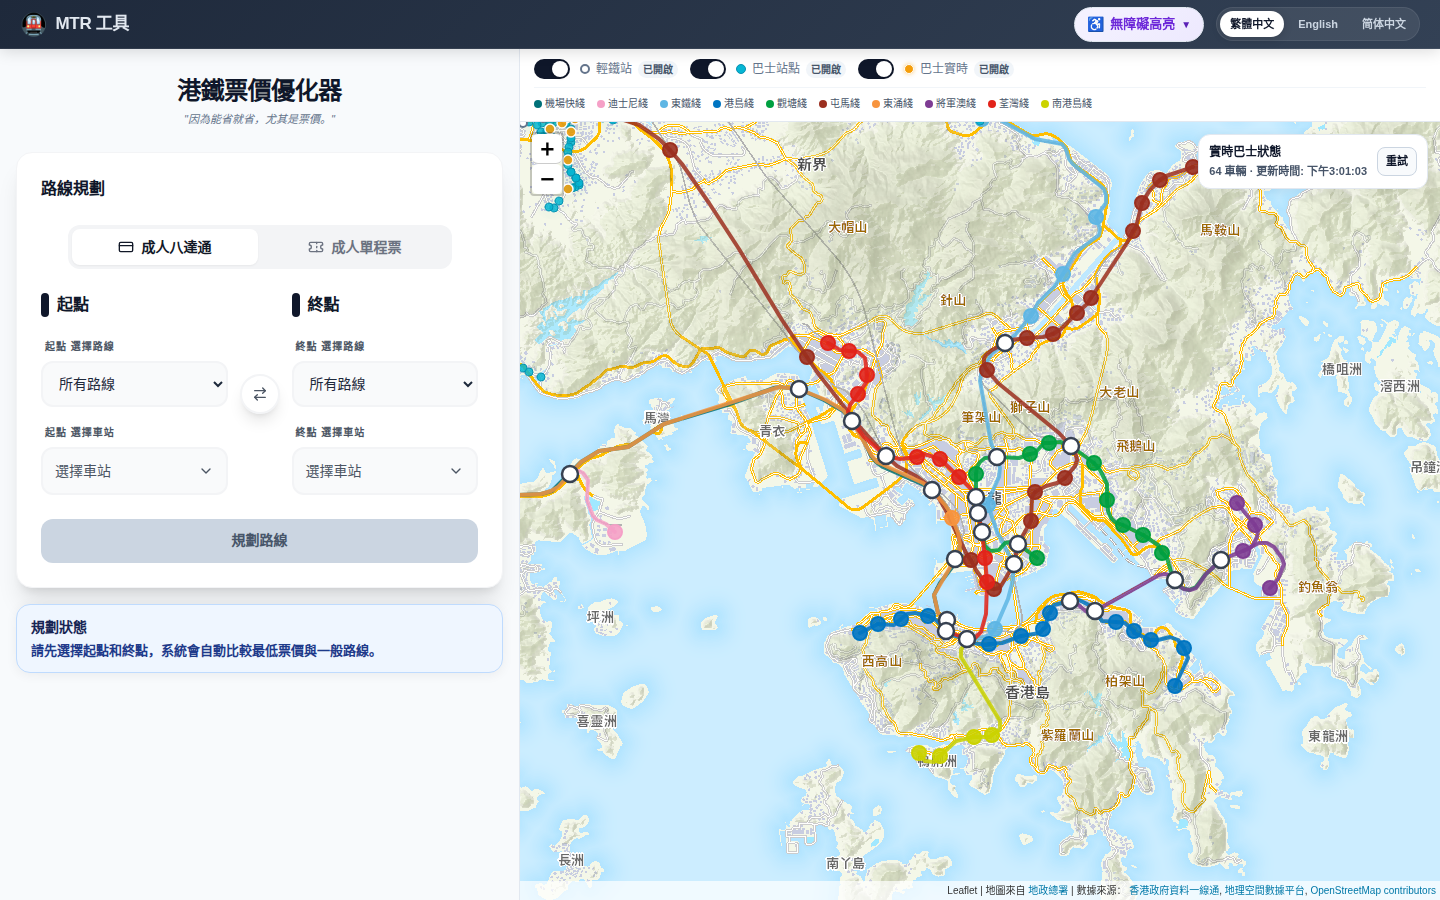
\includegraphics[width=\linewidth,height=0.72\textheight,keepaspectratio]{desktop-map-overview.png}
    \end{column}
    \begin{column}{0.36\textwidth}
      \begin{itemize}
        \item 左侧：票种、起点、终点、规划状态和路线结果。
        \item 右侧：真实地图、线路、站点、轻铁、巴士站和实时巴士。
        \item 用户不需要在表单页和地图页之间切换。
      \end{itemize}
      \hciprinciple{尼尔森启发式“系统状态可见性”：输入状态、地图状态和路线结果并列呈现。}
    \end{column}
  \end{columns}
\end{frame}

\begin{frame}{路线结果展示：让用户敢按推荐走}
  \begin{columns}[T,onlytextwidth]
    \begin{column}{0.46\textwidth}
      \begin{block}{展示的信息}
        \begin{itemize}
          \item 最低票价、常规票价、节省金额
          \item 出入闸次数、线路名称、站点序列
          \item 起点、终点、出闸再入闸点的地图高亮
        \end{itemize}
      \end{block}
      \begin{block}{用户价值}
        省钱方案通常涉及额外出入闸，界面需要同时展示节省金额和操作代价。
      \end{block}
    \end{column}
    \begin{column}{0.50\textwidth}
      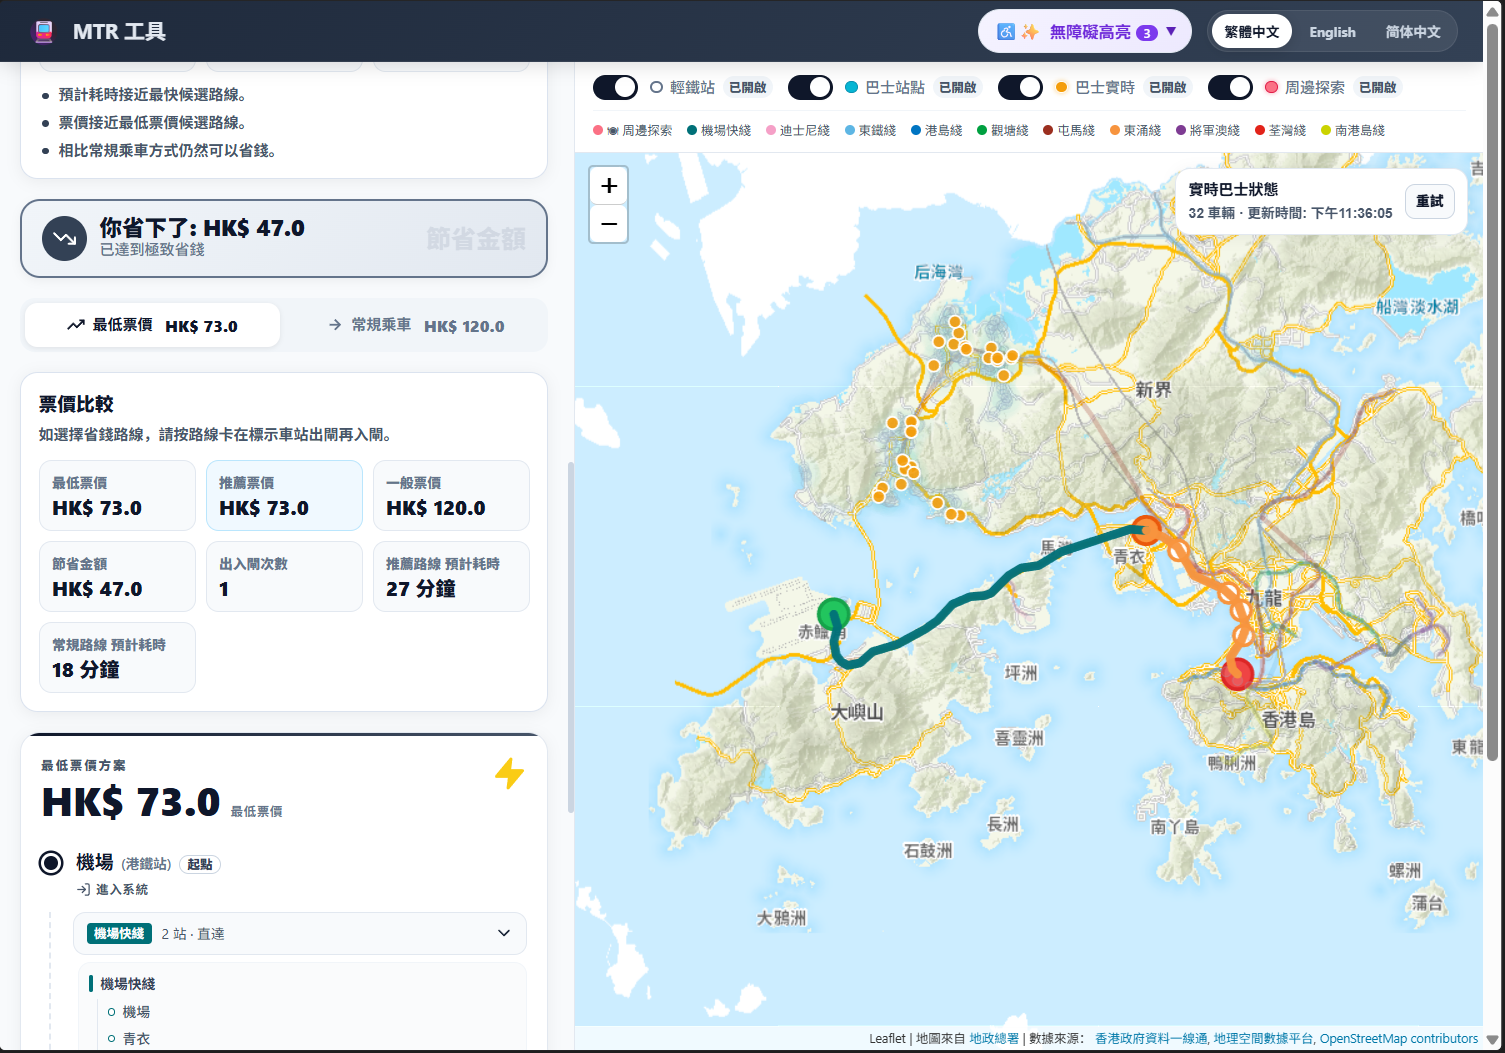
\includegraphics[width=\linewidth,height=0.70\textheight,keepaspectratio]{route-savings-fanqi.png}
    \end{column}
  \end{columns}
  \hciprinciple{诺曼“反馈”原则：操作后立即显示票价、路线、节省金额和地图高亮。}
\end{frame}

\begin{frame}{移动端适配：地图优先与底部面板}
  \begin{columns}[T,onlytextwidth]
    \begin{column}{0.27\textwidth}
      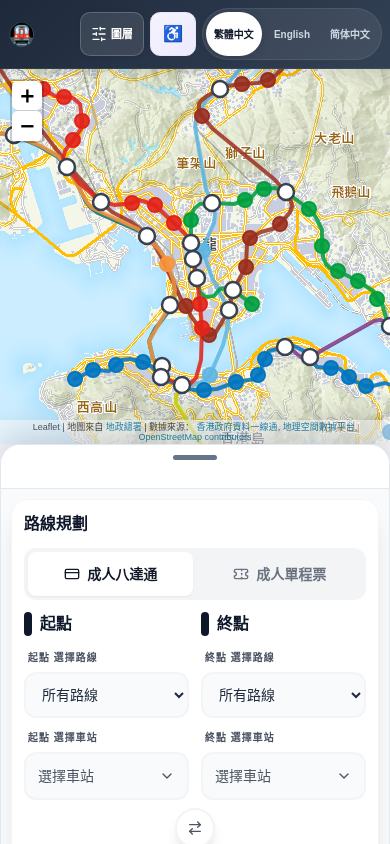
\includegraphics[width=\linewidth,height=0.72\textheight,keepaspectratio]{mobile-overview.png}
    \end{column}
    \begin{column}{0.27\textwidth}
      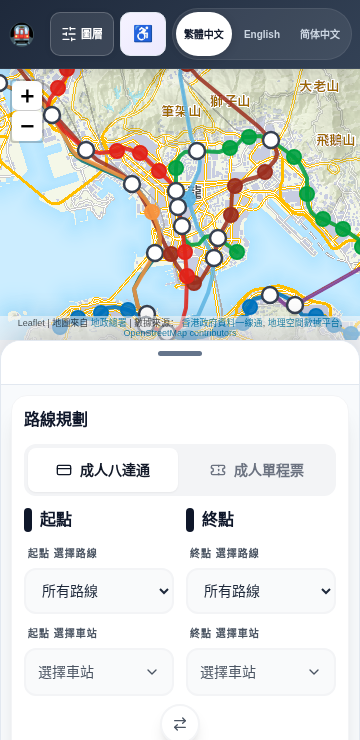
\includegraphics[width=\linewidth,height=0.72\textheight,keepaspectratio]{mobile-narrow.png}
    \end{column}
    \begin{column}{0.42\textwidth}
      \begin{itemize}
        \item 手机出行场景中，地图和方向感优先于长表单。
        \item 路线规划放入底部面板，支持展开、收起和拖拽。
        \item 窄屏下处理按钮、图层、表单之间的遮挡和误触。
        \item 线路颜色、图层开关和图例降低复杂地图的信息负担。
      \end{itemize}
      \hciprinciple{Fitts 定律与用户控制：移动端把高频控件放在易触达区域，并允许面板展开/收起。}
    \end{column}
  \end{columns}
\end{frame}

\begin{frame}{第三部分：周边旅游推荐}
  \speakerline{郎若谷}{2351871}
  \begin{block}{负责内容}
    站点周边景点与美食推荐：回答用户“到站之后吃什么、逛什么、怎么走过去”。
  \end{block}
  \hciprinciple{场景化设计：围绕用户完整旅程设计，而不只覆盖单个查询动作。}
\end{frame}

\begin{frame}{周边数据：真实、可缓存、可溯源}
  \begin{columns}[T,onlytextwidth]
    \begin{column}{0.50\textwidth}
      \begin{block}{离线数据管线}
        \begin{itemize}
          \item OpenStreetMap：餐饮与景点位置
          \item Wikidata / Wikimedia：图片、简介、授权信息
          \item Apify 抓取结果：评分、评论数、价位等补充信号
          \item 构建期生成本地 \texttt{pois.json} 和图片资源
        \end{itemize}
      \end{block}
    \end{column}
    \begin{column}{0.46\textwidth}
      \begin{block}{当前覆盖}
        \begin{itemize}
          \item 约 96 个车站
          \item 2500+ 个 POI
          \item 2100+ 张本地图片
          \item 前端运行时零外网依赖
        \end{itemize}
      \end{block}
      \hciprinciple{可用性中的效率与可信度：减少等待时间，并标明信息来源以支持用户判断。}
    \end{column}
  \end{columns}
\end{frame}

\begin{frame}{周边探索交互：从列表到可走路线}
  \begin{columns}[T,onlytextwidth]
    \begin{column}{0.48\textwidth}
      \begin{block}{探索面板}
        \begin{itemize}
          \item 类别：全部 / 美食 / 景点
          \item 排序：推荐、距离、评分
          \item 半径、菜系、收藏、随机推荐
          \item 空态给出“扩大半径”的可执行建议
        \end{itemize}
      \end{block}
    \end{column}
    \begin{column}{0.48\textwidth}
      \begin{block}{地图与路线}
        \begin{itemize}
          \item POI 卡片与地图标记双向联动
          \item 卡片采用渐进式披露：扫读信息先显示，详情按需展开
          \item 收藏多个点后生成最近邻“逛吃路线”
        \end{itemize}
      \end{block}
    \end{column}
  \end{columns}
  \hciprinciple{渐进式披露与用户控制：先展示决策必需信息，详情和筛选按需展开。}
\end{frame}

\begin{frame}{第四部分：用户关怀}
  \speakerline{樊祺}{2350262}
  \begin{block}{负责内容}
    无障碍设施信息、无障碍友好路线偏好、用户体验调研与竞品分析。
  \end{block}
  \hciprinciple{通用设计与包容性设计：让不同能力、语言和出行偏好的用户都能完成任务。}
\end{frame}

\begin{frame}{无障碍设施：从“能到达”到“适合我到达”}
  \begin{columns}[T,onlytextwidth]
    \begin{column}{0.49\textwidth}
      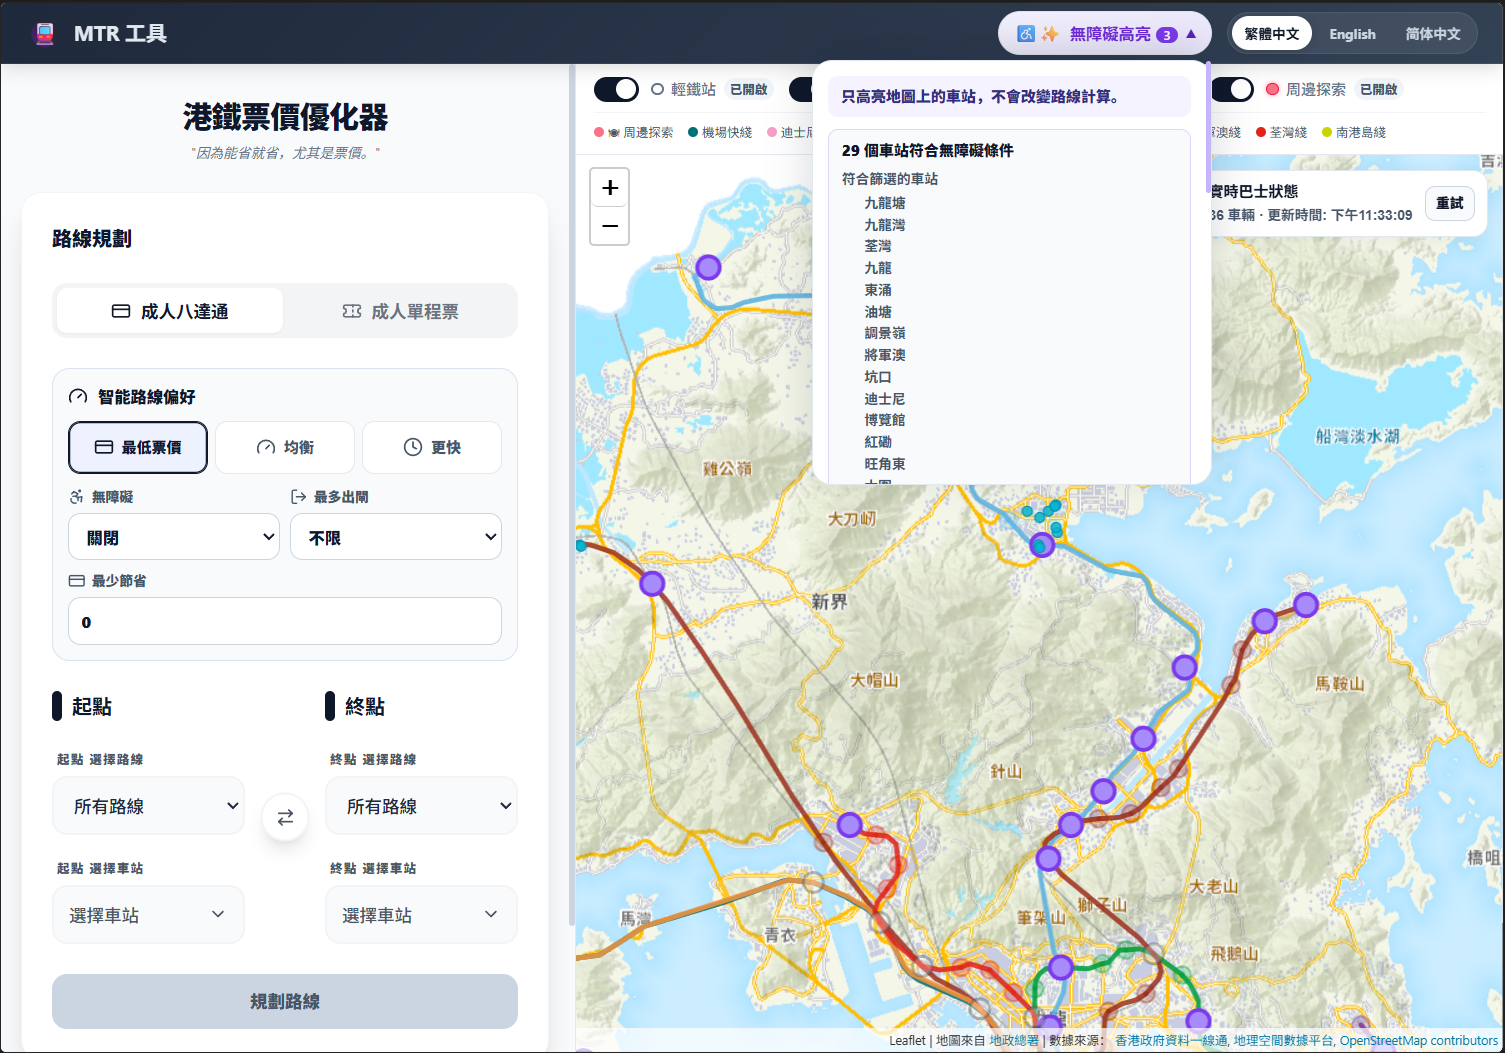
\includegraphics[width=\linewidth,height=0.68\textheight,keepaspectratio]{accessibility-filter.png}
    \end{column}
    \begin{column}{0.49\textwidth}
      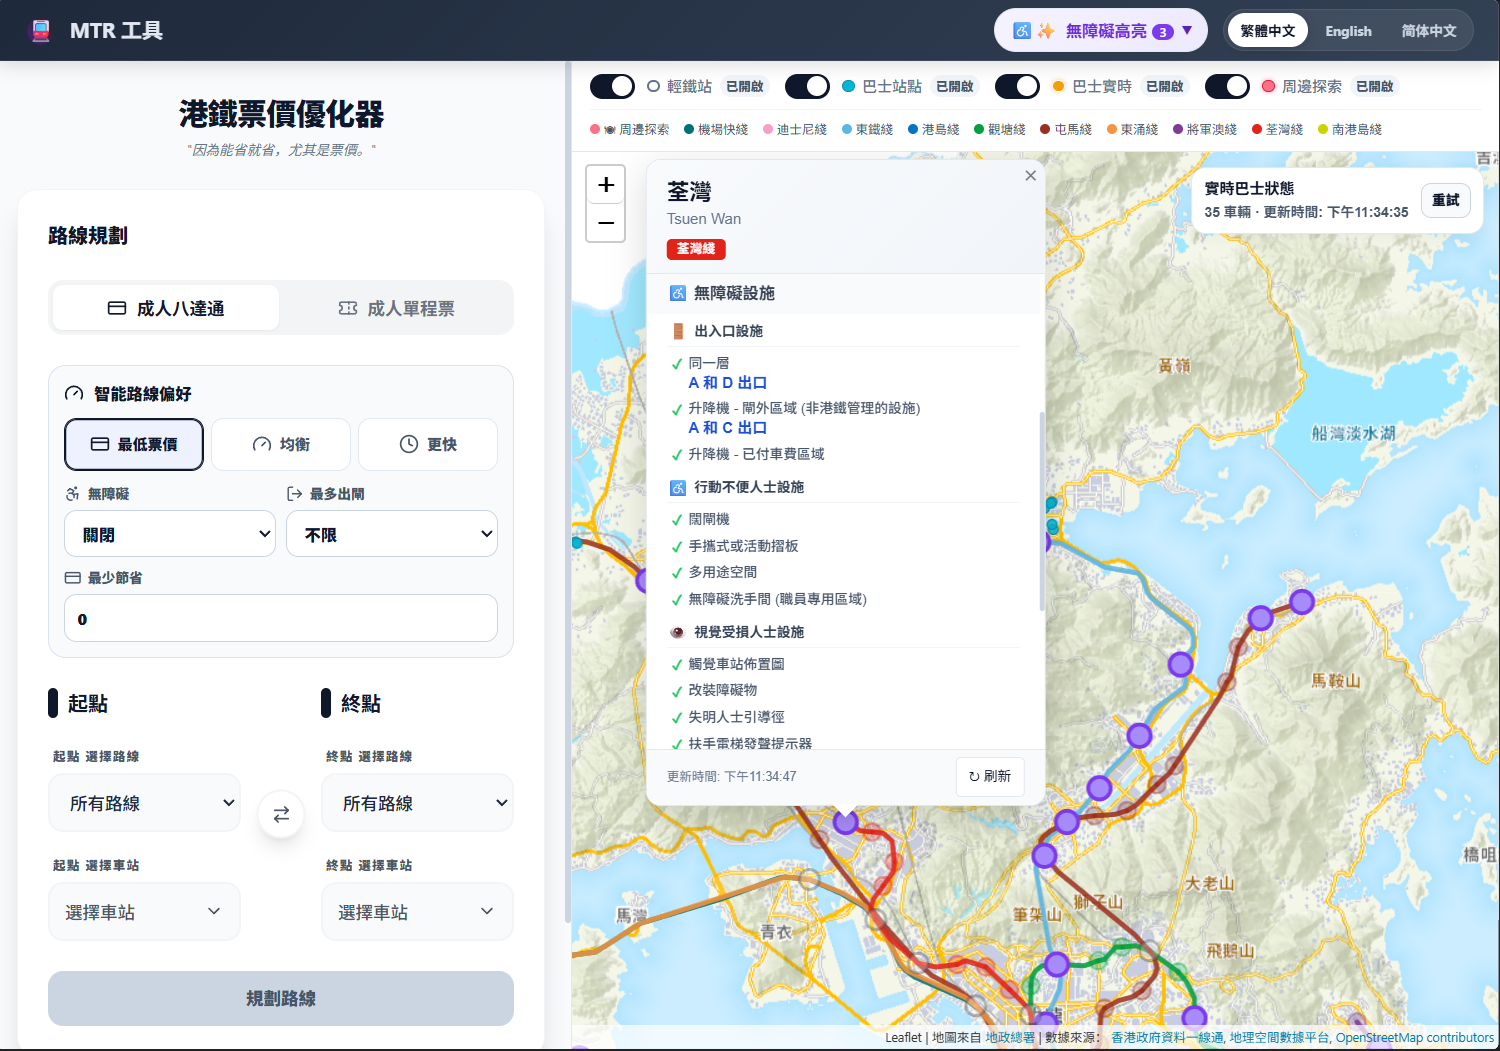
\includegraphics[width=\linewidth,height=0.68\textheight,keepaspectratio]{accessibility-popup.png}
    \end{column}
  \end{columns}
  \vspace{0.3em}
  \small
  地图可按无障碍条件高亮车站；车站详情展示出入口、电梯、轮椅设施、视听辅助等信息。
  \hciprinciple{WCAG 可感知原则与通用设计：把无障碍设施显式呈现，减少出行前的不确定性。}
\end{frame}

\begin{frame}{用户偏好：把“麻烦程度”显式交给用户}
  \begin{columns}[T,onlytextwidth]
    \begin{column}{0.47\textwidth}
      \begin{block}{路线偏好}
        \begin{itemize}
          \item 优化目标：最低票价 / 均衡 / 更快
          \item 无障碍策略：关闭 / 优先 / 必须
          \item 最多出闸次数
          \item 最低节省金额阈值
        \end{itemize}
      \end{block}
    \end{column}
    \begin{column}{0.49\textwidth}
      \begin{block}{推荐解释}
        \begin{itemize}
          \item 推荐票价、最低票价、一般票价分开展示
          \item 展示预计耗时、出入闸次数、无障碍匹配度
          \item 当省钱收益不足时回退到更稳妥路线
        \end{itemize}
      \end{block}
    \end{column}
  \end{columns}
  \hciprinciple{尼尔森启发式“用户控制与自由”“错误预防”：让用户定义可接受的出闸和节省阈值。}
\end{frame}

\begin{frame}{用户体验调研：小样本可用性测试}
  \begin{columns}[T,onlytextwidth]
    \begin{column}{0.50\textwidth}
      \begin{block}{测试设置}
        \begin{itemize}
          \item 6 名同学，3 人桌面端、3 人移动端
          \item 任务：罗湖到屯门、解释粉岭分段省钱原因
          \item 任务：找到出闸再入闸点、筛选无障碍车站
          \item 指标：完成率、耗时、错误点、主观满意度
        \end{itemize}
      \end{block}
    \end{column}
    \begin{column}{0.46\textwidth}
      \begin{block}{结果与改进点}
        \begin{itemize}
          \item 路线规划完成率：6/6；平均耗时约 58 秒
          \item 5/6 能正确解释“粉岭出闸再入闸”省钱原因
          \item 4/6 首次能独立找到无障碍筛选入口
          \item 平均满意度：4.3/5；主要建议是加强首次引导
        \end{itemize}
      \end{block}
    \end{column}
  \end{columns}
  \hciprinciple{可用性测试：用任务完成率、耗时、错误和满意度验证界面是否真的可用。}
\end{frame}

\begin{frame}{调研结论与后续改进}
  \begin{columns}[T,onlytextwidth]
    \begin{column}{0.48\textwidth}
      \begin{block}{调研结论}
        \begin{itemize}
          \item 路线规划任务完成率高，说明主流程可用
          \item 粉岭分段案例能帮助用户理解票价优化
          \item 地图高亮能降低寻找出闸点和设施点的成本
          \item 无障碍筛选入口仍需要更明显的首次提示
        \end{itemize}
      \end{block}
    \end{column}
    \begin{column}{0.48\textwidth}
      \begin{block}{后续改进}
        \begin{itemize}
          \item 在首次使用时解释“出闸再入闸”和“最低节省金额”
          \item 给无障碍筛选和图层按钮增加更明确的视觉提示
          \item 在路线卡片中继续突出费用、次数和设施匹配度
          \item 扩展更多真实用户样本，验证老人、游客和行动不便用户场景
        \end{itemize}
      \end{block}
    \end{column}
  \end{columns}
  \vspace{0.6em}
  \centering
  \Large \textcolor{MTRBlue}{欢迎访问 GitHub 开源项目与在线部署版本继续体验。}
\end{frame}

\end{document}
